%%%%%%%%%%%%%%%%%%%%%%%%%%%%%%%%%%%%%%%%%%%%%%%%%%%%%%%%%%%%%%%%%%%%%%%%%%%%%%%
% intro.tex: Introduction to the thesis
%%%%%%%%%%%%%%%%%%%%%%%%%%%%%%%%%%%%%%%%%%%%%%%%%%%%%%%%%%%%%%%%%%%%%%%%%%%%%%%%
\chapter{Mathematical formulation}
\label{math_chapter}
%%%%%%%%%%%%%%%%%%%%%%%%%%%%%%%%%%%%%%%%%%%%%%%%%%%%%%%%%%%%%%%%%%%%%%%%%%%%%%%%

\section{Governing Equations}
\subsection{VLE-based CFD framework}
\label{sec:model:cfd}
%In this study, a transcritical multiphase flow solver is developed by coupling a density-based fully compressible CFD solver with several VLE solvers. 
The governing equations of the CFD solver are the multi-component transport equations, including the mixture density equation (i.e., continuity equation), mixture momentum equations, mixture internal energy equation, and component mass fraction equation as follows:
\begin{align}
 &\frac{\partial \rho}{\partial t}+\frac{\partial \rho u_i}{\partial x_i}=0 \label{Gc},\\
 &\frac{\partial \rho u_i}{\partial t}+\frac{\partial \rho u_i u_j}{\partial x_j}=-\frac{\partial P}{\partial x_i}+\frac{\partial \tau_{ij}}{\partial x_j} \label{Gm},\\
 &\frac{\partial \rho e}{\partial t}+\frac{\partial \rho u_i e}{\partial x_i}+\frac{\partial \rho K}{\partial t}+\frac{\partial \rho u_i K}{\partial x_i}+\frac{\partial  u_i P}{\partial x_i}=-\frac{\partial q_i}{\partial x_i} +\frac{\partial \tau_{ij}u_j}{\partial x_i},\\
  &\frac{\partial \rho Y_m}{\partial t}+\frac{\partial \rho Y_m u_i}{\partial x_i}=\frac{\left(\rho Y_m V_{mi}\right)}{\partial x_i},
  %\frac{\partial }{\partial x_j}\left(\rho D \sum_m h_m \frac{\partial Y_m}{\partial x_j}\right)-\frac{\partial }
\end{align}
where $u_i$ is the velocity, $\rho$ is mixture density, $e$ is specific internal energy, $Y_m$ is the mass fraction of specie $m$, $\tau_{ij}$ is the viscous stress tensor defined by $ \tau_{ij} = -\frac{2}{3}\mu\frac{\partial u_k}{\partial x_k}\delta_{ij} + \mu \left( \frac{\partial u_i}{\partial x_j} +\frac{\partial u_j}{\partial x_i}\right) $, $K$ is the kinetic energy, and $q_i$ is the heat flux. $q_i = -\kappa \nabla  T$ where $\kappa$ is the thermal conductivity. 
The Fickian diffusion is used to evaluate the diffusion velocity in the governing equations:

$$ V_{mi} = -\frac{D_m}{X_m}\frac{\partial X_m} {\partial x_i} + \sum^{N}_{s}\frac{Y_s D_s}{X_s}\frac{\partial X_s} {\partial x_i},$$
where $X_m$, and $D_m$ are the mole fraction and the mixture-averaged diffusion coefficient of specie $m$, respectively. The second correction term is to ensure global mass conservation $\sum^{N}_{m} \rho Y_m V_m = 0$.

\textbf{Fully compressble solver}
The CFD solver was developed based on the central-upwind scheme \cite{kurganov2001semidiscrete,greenshields2010implementation}. At each time step, the conservative variables $\rho$, $\rho u$, $\rho e$, and $\rho Y_m$ are updated according to the governing equations. The central upwind scheme mentioned is a fully conservative (FC) method. 

To eliminate spurious pressure oscillations, a quasi-conservative approach called the double flux (DF) method \cite{abgrall2001computations,billet2003adaptive,ma2017entropy} is also implemented.
This method locally freezes the real fluid properties to those of an equivalent calorically perfect gas. During the calculation of the new time step, in each cell, a local calorically perfect-gas EOS is defined using the thermodynamic properties. The pressure field is updated using this newly defined EOS, effectively mitigating the occurrence of spurious pressure oscillations. Subsequently, the remaining thermodynamic properties such as density and species mass fraction are updated using the real-gas EOS and PV flash based on the updated pressure, density, and species mass fraction values. The use of a calorically perfect-gas EOS in the double flux method has been shown by Ma et al. to successfully remove spurious pressure oscillations \cite{ma2017entropy}. To define a locally calorically perfect-gas EOS, an effective specific heat ratio $\gamma^*$ and an effective internal energy $e_0^*$  are formulated as:
\begin{align}
\gamma^*& = \frac{\rho c^2}{P},&e_0^*&= e-\frac{Pv}{\gamma^*-1},
\end{align}
where $c$ is the speed of sound, and $v$ is the specific volume. %$\gamma^*$ and $e_0^*$ can be calculated from the density, internal energy, and speed of sound, which are obtained from real gas EOS.
With real-fluid EOS, $\gamma^*$ and $e_0^*$ can be nonlinear functions of the thermodynamic states and may not be constant. The main idea of the double flux method is to freeze $\gamma^*$ and $e_0^*$ in space during each time step advancement. When calculating a flux of a face of a certain cell, the state variable used is not directly from the cell values but reconstructed using $\gamma^*$, $e_0^*$, $P$, and $\rho$. Although this face also belongs to the adjacent cell, its $\gamma^*$, $e_0^*$ of the adjacent cell are not used.  For example, on a one-dimensional mesh, the numerical face flux $F^L_{i+\frac{1}{2}}$ for the cell $i$ at $x_{i+\frac{1}{2}}$ can be expressed as (see Fig.~\ref{DF_CFD})
\begin{align}
F^L_{i+\frac{1}{2}}& = F\left(U^L_{i+\frac{1}{2}},U^R_{i+\frac{1}{2}}\right),&
U^L_{i+\frac{1}{2}}& = U^L\left(\gamma^*_i,e_{0,i}^*,P,\rho ,Y\right),&
U^R_{i+\frac{1}{2}}& = U^R\left(\gamma^*_i,e_{0,i}^*,P,\rho ,Y\right),
\end{align}
where $U^L$ and $U^R$ are conservative variables constructed using calorically perfect-gas EOS. The stencil for constructing conservative variables depends on the interpolation scheme, and the vanLeer method \cite{van1974towards} is used in the current work. In the central-upwind method,

\begin{align} F^L_{i+\frac{1}{2}} &= \alpha u^LU^L + \left(1-\alpha\right)u^R U^R + \omega \left(U^R-U^L\right),&
\alpha &= \frac{\phi^L}{\phi^L +\phi^R},&
 \omega &= \alpha \left(1-\alpha\right) \left(\phi^L+\phi^R\right)
 \end{align}
\begin{align} \phi^L& = max\left(c^L+|u^L|,c^R + |u^R|,0\right),&\phi^R &= max\left(c^L-|u^L|,c^R - |u^R|,0\right)
\end{align}

where $c$ and $u$ are the speed of sound and velocity respectively. They are obtained from the same interpolation scheme.


In this way, the $\gamma^*$ and $e_0^*$ are frozen, and the fluid is locally calorically perfect to remove spurious pressure oscillation. 
Since each face is adjacent to two cells, the two fluxes (i.e., the left flux $F^L_{i+\frac{1}{2}}$ and the right flux $F^R_{i+\frac{1}{2}}$ in Fig.~\ref{DF_CFD}) obtained from two cells can be different. That is why this method is called ``double flux'', and where two fluxes are different, the numerical scheme is no more conservative. 
\begin{figure*}[htbp]
\centering
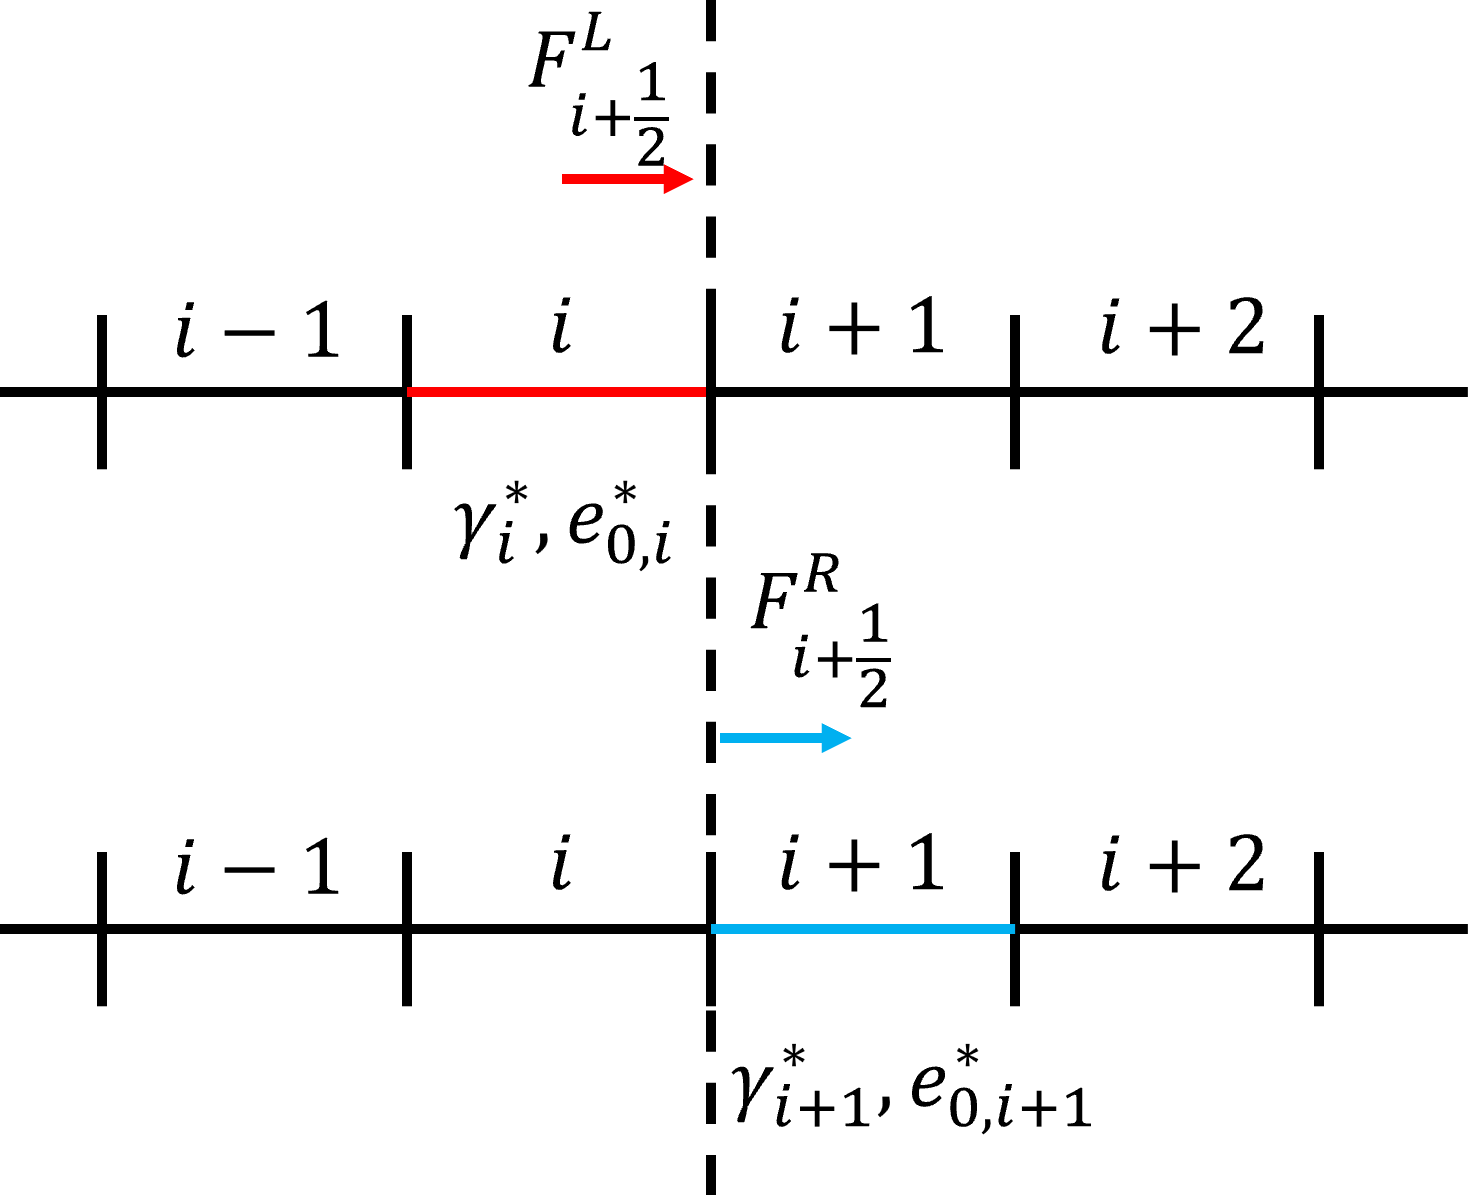
\includegraphics[width=0.4\linewidth]{DF.png}
\caption{Schematic of the double flux (DF) method in a one-dimensional mesh.}
\label{DF_CFD} 
\end{figure*}

At each time step, $\rho$, $u$, and $Y_m$ are updated using the central-upwind scheme. Then, the DF method is used to update $e$ and $P$. After that, $T,\beta,c$ are obtained using the PV flash solver. For the fully conservative scheme (without DF method), $P,T,\beta,c$ are directly updated using the UV flash solver. This entire process is shown in Fig.~\ref{FC_CFD}. DF method is useful to solve the system with large density gradient, but since it is not an energy-conservative scheme, it could cause other problems. In Sec.~\ref{sec:DF}, we compared the results of two methods, and discuss their pros and cons.

\begin{figure*}[htbp]
\centering
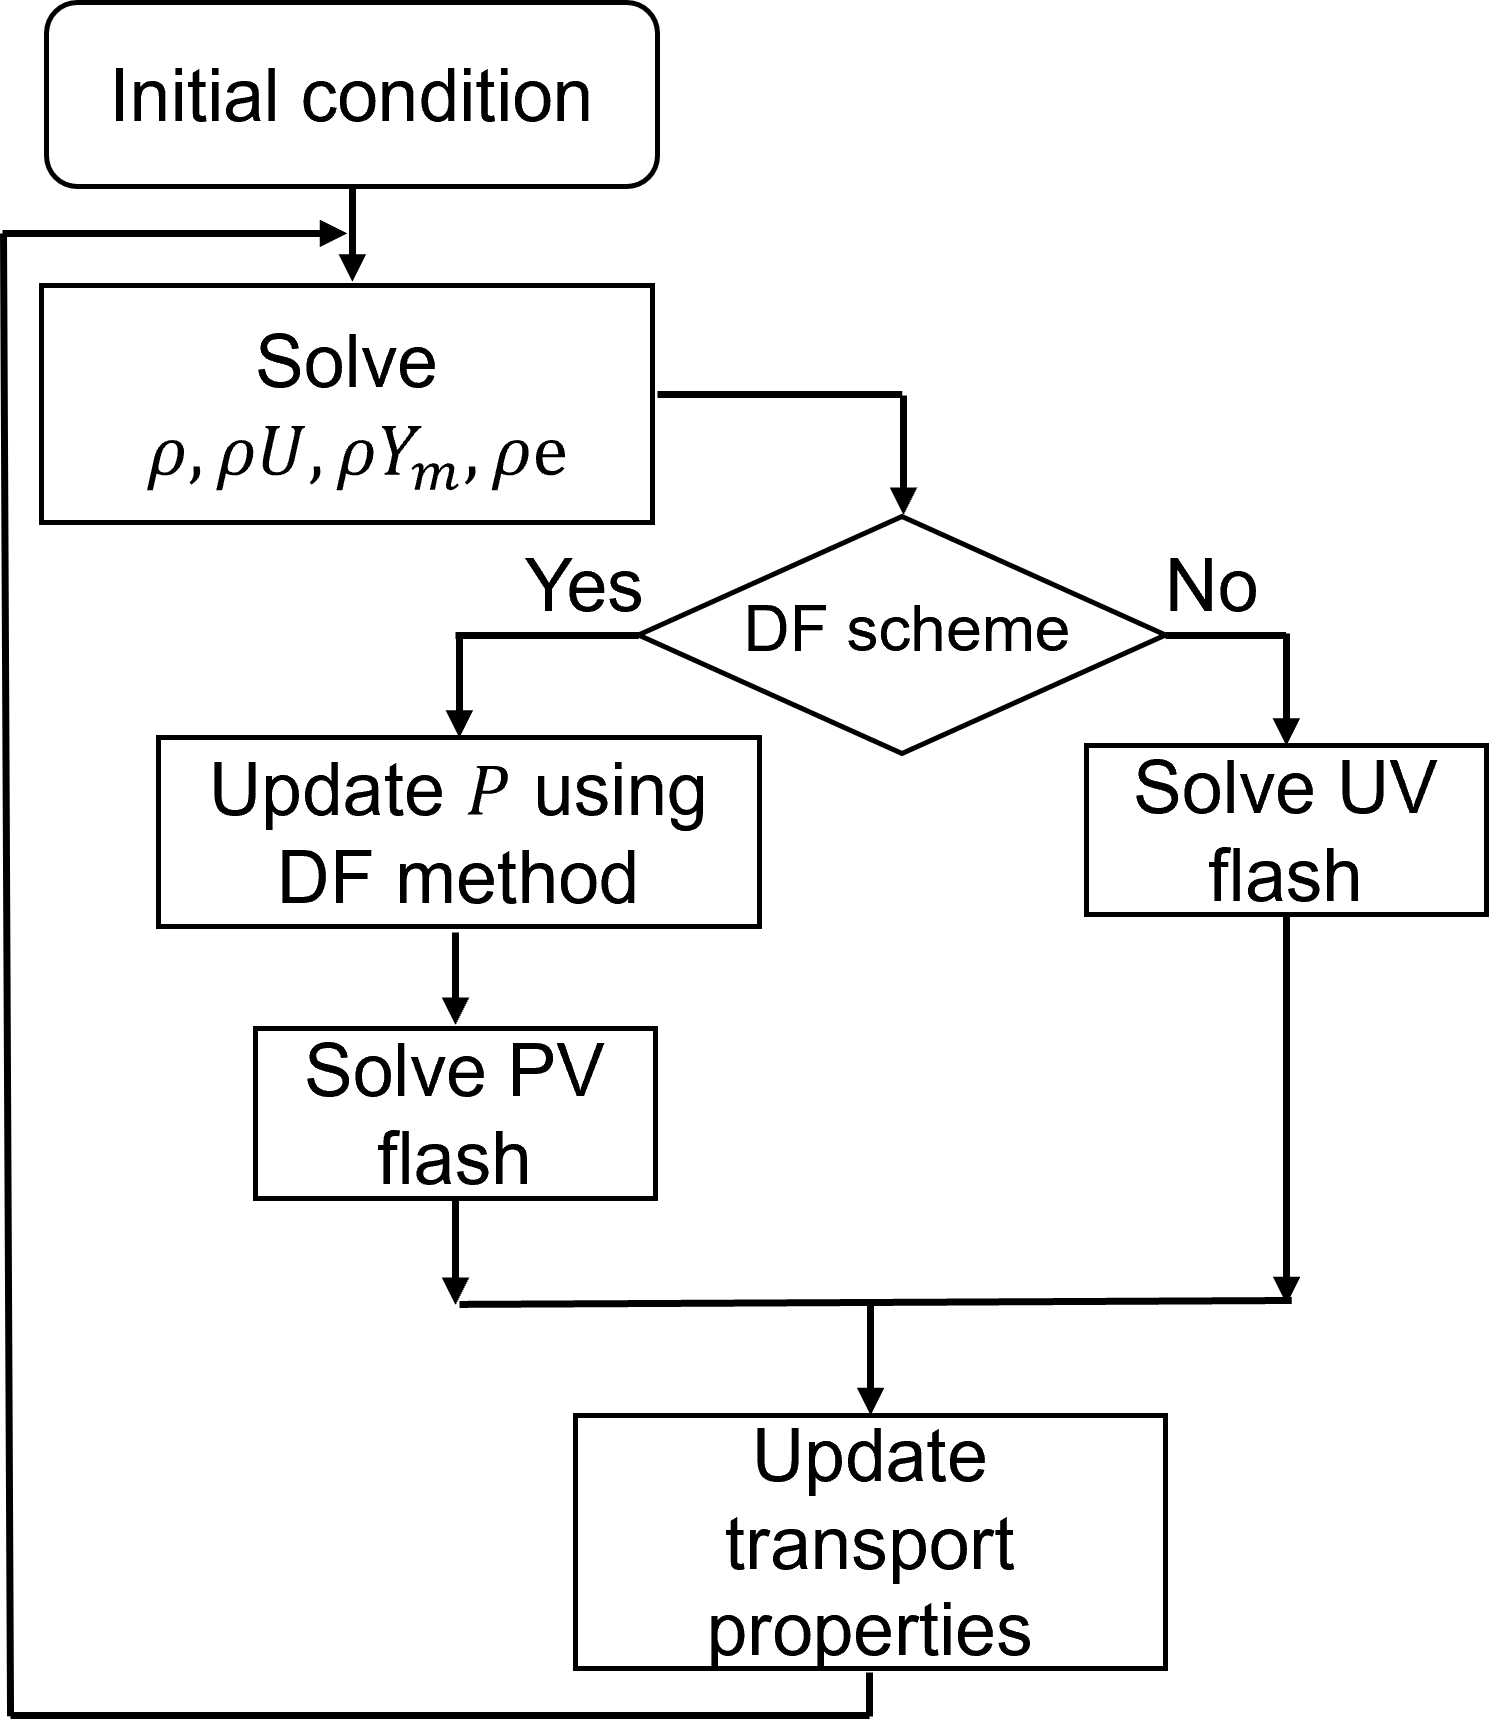
\includegraphics[width=0.4\linewidth]{solver_flow_chart.png}
\caption{Flow chart of the VLE-based CFD framework.}
\label{FC_CFD} 
\end{figure*}

\textbf{PISO solver}

In this study, a high-pressure multiphase flow simulation framework is developed by coupling a pressure-based CFD solver with a VLE solver (the HPn flash): i.e., a VLE-based CFD simulation framework. %The compressible solver used in this research, is the sprayFoam solver in OpenFOAM, an open source C++ library based on the Finite Volume Method. 
The CFD solver is based on multicomponent governing equations, including the continuity equation, mixture momentum equations, mixture specific internal enthalpy equation, and transport equations of distinct components in the mixture, as follows:
\begin{align}
     & \frac{\partial \rho}{\partial t}+\frac{\partial \rho u_i}{\partial x_i}=0 \label{G:start}                                                                                                                                                                            \\
     & \frac{\partial \rho u_i}{\partial t}+\frac{\partial \rho u_i u_j}{\partial x_j}=-\frac{\partial p}{\partial x_i}+\frac{\partial \tau_{ij}}{\partial x_j} \label{Gm}                                                                                                   \\
     & \frac{\partial \rho h}{\partial t}+\frac{\partial \rho u_i h}{\partial x_i}+\frac{\partial \rho K}{\partial t}+\frac{\partial \rho u_i K}{\partial x_i}-\frac{\partial p}{\partial t}=-\frac{\partial q_i}{\partial x_i} +\frac{\partial \tau_{ij}u_j}{\partial x_i} \\
     & \frac{\partial \rho Y_m}{\partial t}+\frac{\partial \rho Y_m u_j}{\partial x_i}=\frac{\partial }{\partial x_j}\left(\rho \sum_m D_m \frac{\partial Y_m}{\partial x_j}\right) \label{G:end}
\end{align}
where $u_i$ is the velocity, $\rho$ and $h$ are the mixture density and internal enthalpy, respectively, $Y_m$ is the mass fraction of component $m$, $p$ is the pressure, $\tau_{ij}$ is the viscous stress tensor, $K$ is the kinetic energy, $q_i$ is the heat flux, and $D_m$ is the mass diffusivity of component $m$.
In this study, $q_i=-\alpha \nabla h$ where $\alpha$ is the thermal diffusivity. In the relevant systems of this study (mixture: \ce{CH4}/\ce{CO2}/\ce{H2O}, \ce{O2}/\ce{CO2}/\ce{H2O}; $p$: $10^7$ Pa; $T$: 300-700 K), the Lewis numbers ($Le_m=\alpha/D_m$) are obtained using the models mentioned in Sec.~\ref{thermo models}, and their values are in the range of $O(10^3)$ $\sim$ $O(10^5)$. Hence, the contribution of mass diffusion to energy flux is weak, and it is neglected in this study.

The OpenFOAM solver uses the PIMPLE algorithm ~\cite{holzmann2016mathematics}, which is a combination of the SIMPLE (semi-implicit method for pressure-linked equations) \cite{patankar1983calculation} and PISO (pressure-implicit split-operator) algorithms \cite{issa1986solution} based on the primitive variables (e.g., pressure $p$). The implementation of the PIMPLE algorithm in OpenFOAM has been validated by a lot of researchers around the world for different thermofluid applications~\cite{robertson2015validation, higuera2014three,gaikwad2019openfoam,gamet2020validation,de2017implementation,ashton2019verification}. Additional validation and verification of the CFD solver are provided in Appendix~\ref{App:vali:CFD}, including two shock tube cases and a jet-in-cross flow case. In the original solver, the SIMPLE algorithm is used to predict $\rho$, $u_i$, $h$, and $Y_m$ from Eqs.~(\ref{G:start}-\ref{G:end}), in every time step (i.e., the outer loop in Fig.~\ref{FC_CFD}). Then, thermodynamic properties, including $T$ (mixture temperature) and $\phi$, are evaluated from the $p$ in the last step and the updated $h$ and $Y_m$ using thermodynamic model. The ideal gas model and Peng-Robinson Equation of State, PR-EOS, are provided in the standard OpenFOAM version. $\phi$ is used to update $p$ and calculate $\rho$. Then, transport properties are updated accordingly. 
Here, $\phi$ is defined as
\begin{align}
     & \phi = \frac{\rho} {p}, \label{EOS}
\end{align}
in which the specific form of $\phi$ depends on the choice of thermodynamics model. Then $p$ is updated iteratively by solving its Poisson equation. Velocity $u_i$ and thermodynamic properties ($\rho$, $T$, $\phi$, etc.) are also updated after solving the pressure equation at each iteration step. This inner iteration is from the PISO algorithm, and hence it is called PISO loop, as shown in Fig.~\ref{FC_CFD}. When PISO loop finshed, $\rho$ is updated using Eq.~(\ref{EOS}). With the updated properties, Eqs.~(\ref{Gm}-\ref{G:end}) are solved iteratively to update $u_i$, $h$, and $Y_m$, respectively, using the semi-implicit method (i.e., the predictor step) until it converges. This iteration is from the SIMPLE algorithm, and hence is called SIMPLE loop, as shown in Fig.~\ref{FC_CFD}. When SIMPLE loop finished, the next time step starts.


\begin{figure}[htbp]
    \centering
    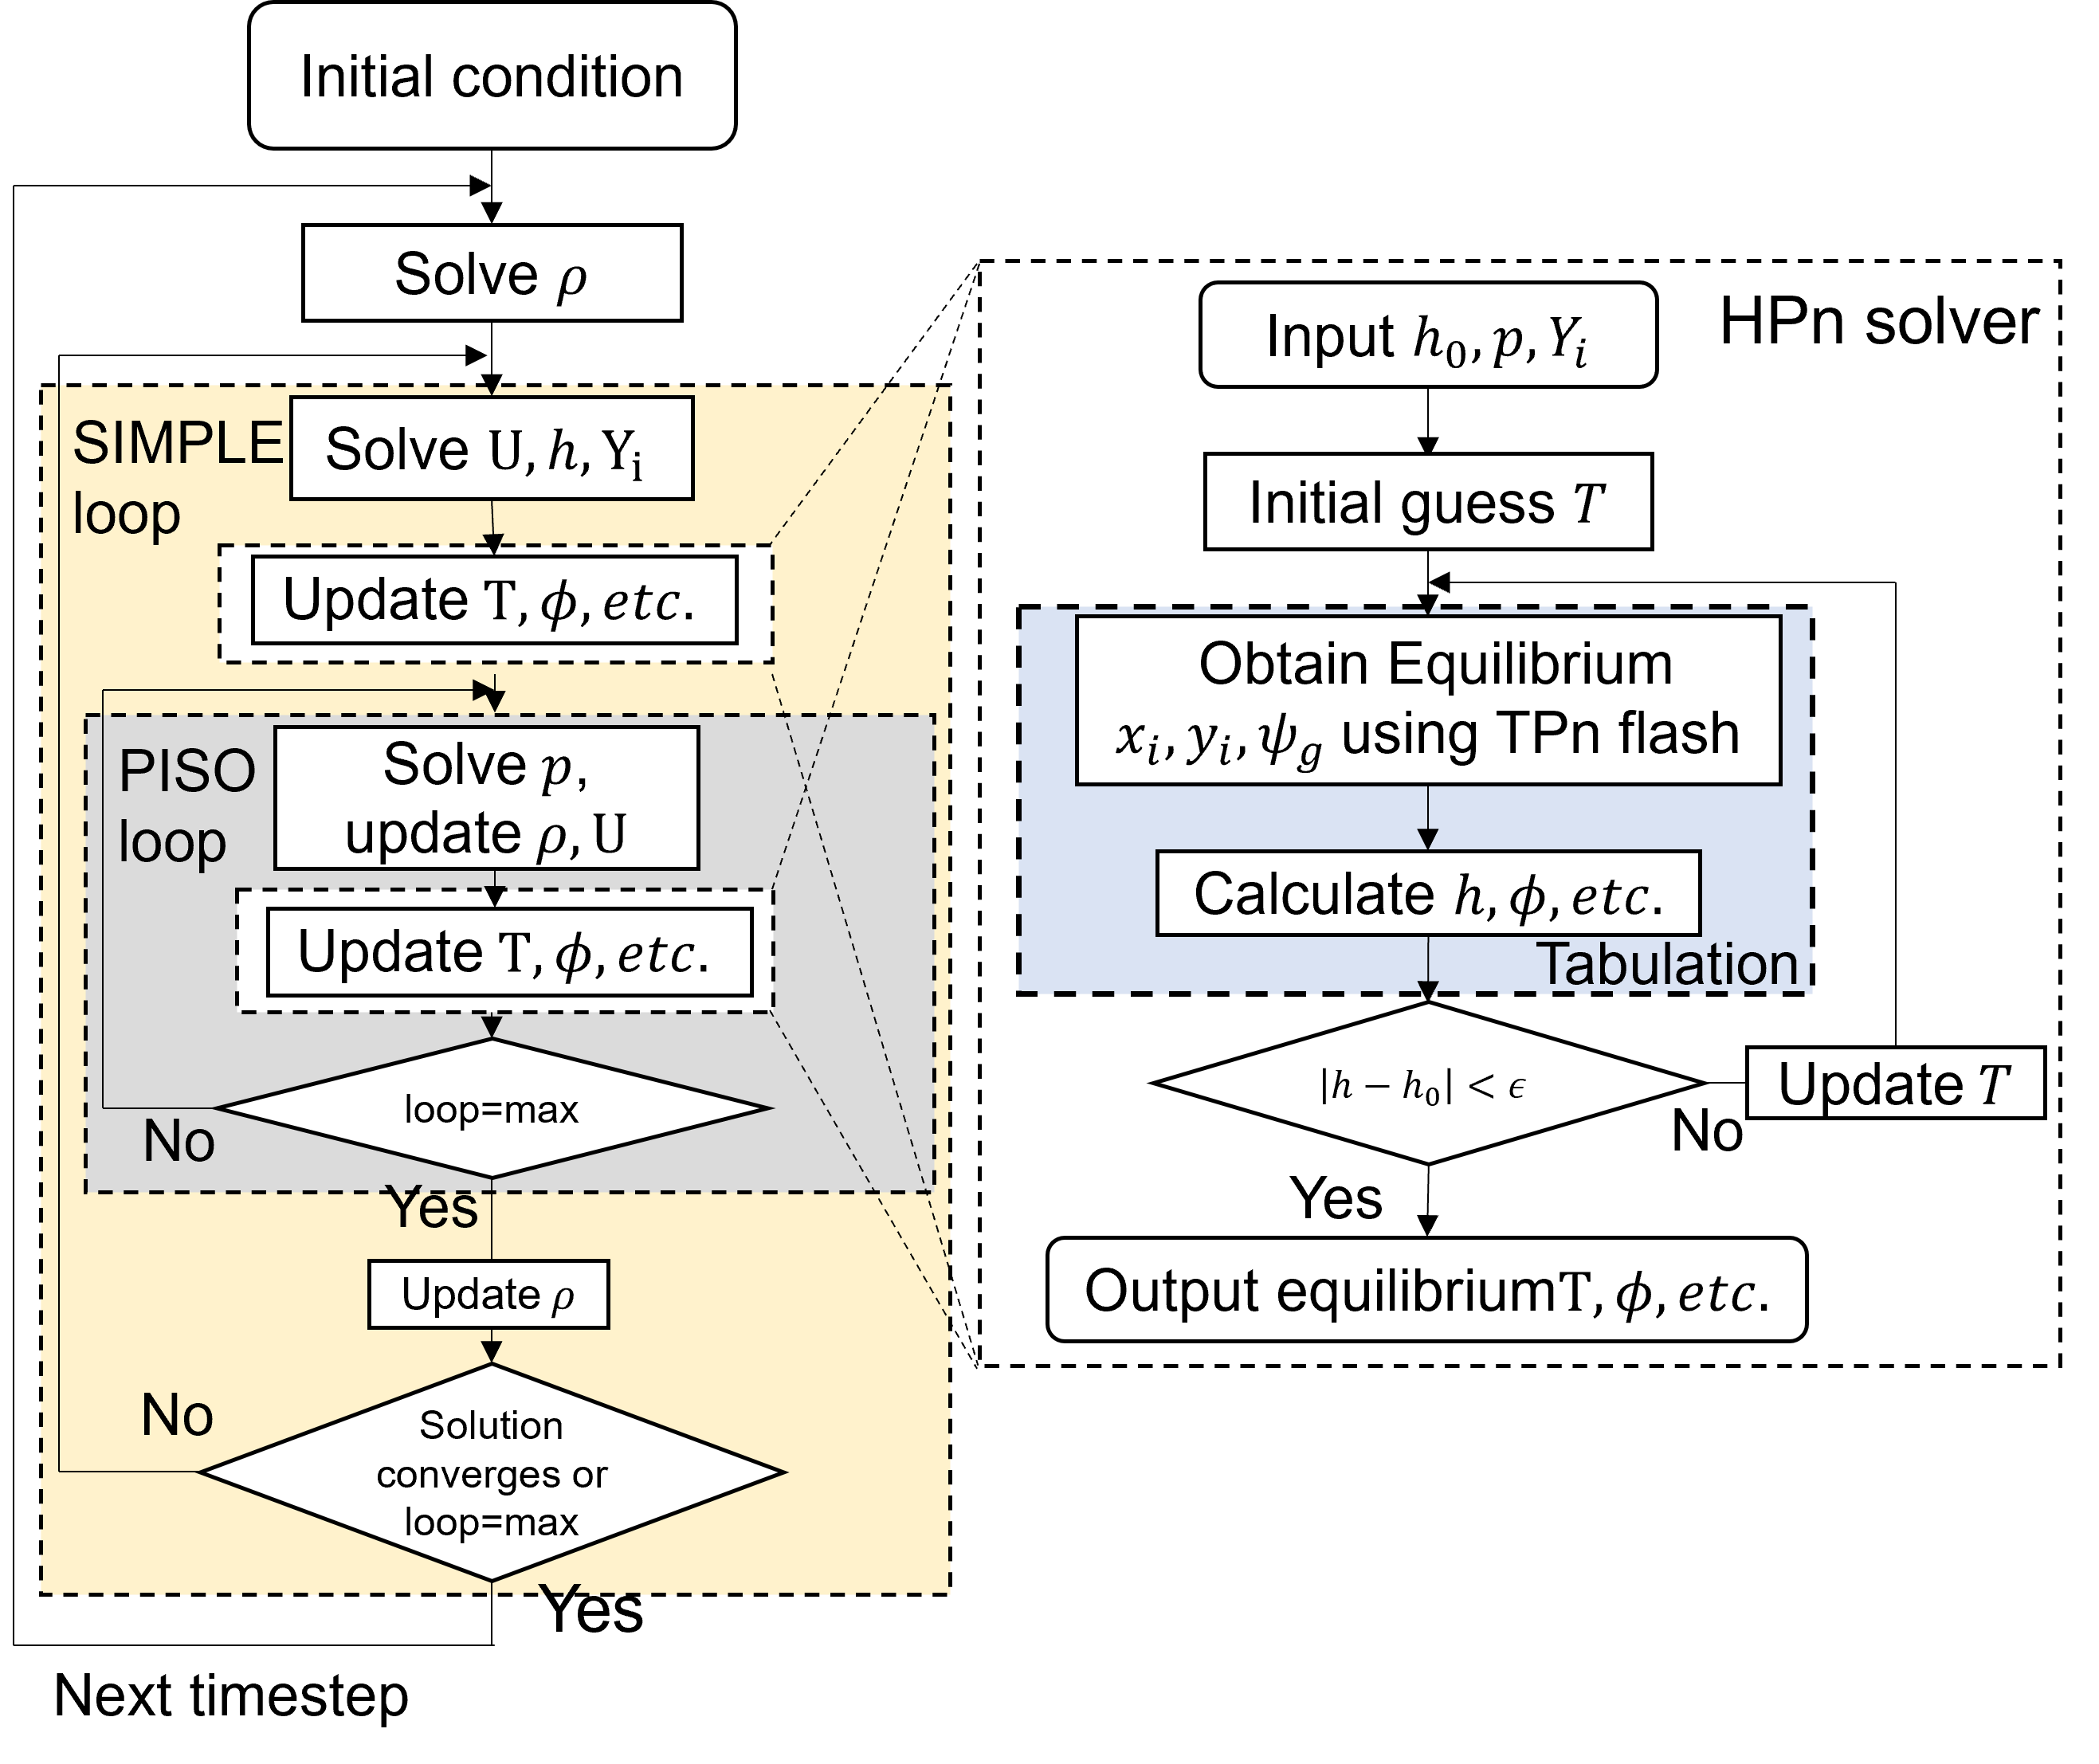
\includegraphics[width=0.95\linewidth]{flowchart.png}
    \centering
    \caption{Flow chart of the VLE-based CFD solver.}
    \label{FC_CFD}
\end{figure}

The new contributions from this study to the OpenFOAM solver and PIMPLE algorithm are summarized here. This study replaces the original thermodynamic model with the VLE + PR-EOS model implemented in this study, as shown in Fig.~\ref{FC_CFD}. Due to the high computational cost of VLE calculation, a novel VLE-based tabulation method is developed to accelerate simulations and make the CFD solver computationally more affordable, as shown in the right box of Fig.~\ref{FC_CFD}. For each simulation, a table is generated to record the solution of TPn flash, density, enthalpy, $c_p$, and transport properties at different temperatures (280-1200 K), pressures (280-700 bar), and \ce{CO2} mole fractions (0.0001-0.9999). Each solution includes, every species' mole fraction in liquid and gas phases, and transport properties. In simulations, a linear approximation method based on eight neighboring records is used for data retrieval. More details about this VLE-based tabulation method is provided in Appendix~\ref{App:tab}. For a large number of components, this tabulation method will demand infeasible memory, and we are developing a new on-the-fly tabulation of VLE solutions using the \textit{in situ} adaptive tabulation (ISAT) approach~\cite{zhang2021multi}, similar to the idea of correlated dynamic evaluation of real fluid properties for supercritical mixing~\cite{yang2017comparison} and combustion~\cite{milan2019time}.



\section{Models of thermodynamic and transport properties}
In the following, the models of thermodynamic and transport properties are presented. VLE solvers are develped to capture the phase sepeartion  using a cubic EoS. The fundamental VLE theory and VLE solvers' algorithm are presented. And dynamic viscosity, thermal conductivity, and mass diffusivity model for high pressure flow are presented.

\subsection{Peng-Robinson (PR) Equation of State (EOS)}
VLE models require a real-fluid equation of state (EOS) to describe the properties of single phase. Considering the computational efficiency, acceptable accuracy, and simple implementation, the Peng-Robinson (PR) EOS \cite{peng1976new} is used in this study. The PR EOS is formulated as:
\begin{align}
    P=\frac{RT}{V-b}-\frac{a}{V\left(V+b\right)+b\left(V-b\right)}, %\nonumber \\&\left(p=1\rm{: gas};\quad p=2\rm{: liquid}\right)
    \label{eq:preos}
\end{align}
where $R$ is the ideal gas constant, $V$ is molar volume. The energy parameter $a$ and co-volume parameter $b$ for pure component $i$ are formulated as:

\begin{align}
    a_i &= 0.45724\frac{R^2 T_{c_i}^2}{P_{c_i}} \hat{a} , &b_i&=0.07780\frac{RT_{c_i}}{P_{c_i}} \label{eq:ab},\\
    \hat{a}&=\left[1+\kappa\left(1-\sqrt{\frac{T}{T_{c_i}}}\right)\right]^2, &\kappa&=0.37464+1.54226\omega_i-0.26992\omega_i^2,
\end{align}
where $T_{c_i}$ is the critical temperature of component $i$, $P_{c_i}$ is critical pressure of component $i$, and $\omega_i$ is the acentric factor of component $i$. These specie properties are obtained from the NIST REFPROP database. When the PR EOS is used for a multi-component mixture, mixing rules are used to calculate the energy parameter $a$ and co-volume parameter $b$ \cite{reid1977properties}:
\begin{align}
a&=\sum_i\sum_j\chi_i\chi_j\sqrt{a_ia_j}(1-k_{ij}),& b&=\sum_i\chi_i b_i,\label{eq:mix}
\end{align}
where $\chi_i$ is the mole fraction of component $i$, and $k_{ij}$ is the binary interaction parameter which is often obtained by minimizing the deviation between experimental and simulation results. In this work, only \ce{N2}, \ce{n-C8H18}, and \ce{n-C12H26} are involved. The binary interaction parameter of \ce{N2}/\ce{n-C8H18} system and \ce{N2}/\ce{n-C12H26} system are set as 0.1396 and 0.1561, respectively \cite{eliosa2009vapor,garcia2011vapor}. The binary interaction parameter of \ce{n-C8H18}/\ce{n-C12H26} is set as zero.
%where $P$, $R$, $T$ and $V$ are pressure, gas constant, temperature, and specific volume respectively. For single-component fluid, the PR EOS parameters are given by

\subsection{Vapor-Liquid Equilibrium (VLE)}
VLE can determine multi-component mixtures' phase boundaries to capture phase change in transcritical flows. In the VLE theory, the multiphase thermodynamic equilibrium is locally satisfied, which requires the equality of pressure $P$ (i.e., mechanical equilibrium), the equality of temperature $T$ (i.e., thermal equilibrium), and the equality of fugacity $f$ of the two phases for each component $i$ (i.e., chemical equilibrium):
\begin{align}
P_l=P_v=P,\quad T_l=T_v=T,\quad f_{i,l}=f_{i,v},\quad i=1,...,N, \label{eq:eq}
\end{align}
where the subscript `$l$' and `$v$' refer to liquid and vapor, respectively; $f_i$ is the fugacity of component $i$; and $N$ is the number of components.

There are many different types of VLE solvers, such as isothermal-isobaric (TP) flash \cite{michelsen1982isothermal} and isoenergetic-isochoric (UV) flash \cite{saha1997isoenergetic}. All of them need to solve a two-phase system constrained by Eq.~\ref{eq:eq}, together with the mass conservation of each component. To determine the mixture phase properties, in addition to the mole fraction of each component (i.e., the composition of the mixture), two more mixture properties are required. These two properties determine the type of VLE solvers. For example, TP flash uses the mixture temperature (T) and pressure (P) as inputs to solve the system. The VLE solution provides mixture phase properties, including the vapor phase molar fraction $\beta$ and molar fraction of each component in each phase $x_i,y_i$. 

The single-phase thermodynamic properties can be obtained using EOS (including the departure functions derived from EOS) and NASA Polynomials. Additional blend rules are required to bridge the gap between single-phase and two-phase systems. We follow a commonly used method which blends \cite{matheis2018multi,tudisco2020numerical} extensive volume and internal energy, and hence mixture density and mixture specific internal energy are formulated as:
\begin{align} \frac{M}{\rho} = \beta \frac{M_v}{\rho_v}+\left(1-\beta\right)\frac{M_l}{\rho_l}, \label{eq:rho}
\end{align}
\begin{align} Me = \beta M_v e_v + \left(1-\beta\right)M_l e_l, \label{eq:e}
\end{align}
where $M$ is the mixture molar mass, $M_v$ and $M_l$ are vapor phase and liquid phase molar mass, $e$ is specific internal energy. 
Other mixture thermodynamic properties (e.g. mixture enthalpy, mixture specific heat) can be derived based on these properties. 
In this research, TP flash, UV flash, and isobaric-isochoric (PV) flash are applied. Specifically, 
TP flash solves VLE problems with a given temperature (T) and pressure (P), and is used for the initialization step of the CFD simulation; PV flash solves problems with given pressure (P) and specific volume (V), and is used in the double flux (DF) method (in Sec.~\ref{sec:model:cfd}); UV flash solves problems with given internal energy (U) and specific volume (V), and is used in the fully conservative (FC) scheme. 

\textbf{Isothermal and isobaric (TP) flash:}
VLE is governed by fugacity equality Eq.~(\ref{eq:4}) and Rachford-Rice equation~\cite{rachford1952procedure} Eq.~(\ref{eq:5}). Rachford-Rice equation was derived from the mass conservation of each component.
\begin{align}
&f_{i, l}\big/f_{i, g}=1,  \label{eq:4} \\
&\sum_{i=1}^{N}\bigg\{z_i\left(1-K_i\right)\bigg/\left[1+\left(K_i-1\right)\beta\right]\bigg\}=0, \label{eq:5} \\
&\sum_{i=1}^{N}x_i=\sum_{i=1}^{N}y_i=1,  \label{eq:5-2}
\end{align}
where $x_i$ is the mole fraction of component $i$ in liquid phase, $y_i$ is the mole fraction of component $i$ in gas/vapor phase, $z_i$ is the mole fraction of component $i$ in the mixture, $\beta$ is the vapor mole fraction, $K_i$ is the equilibrium constant of component $i$, $K_i=y_i/x_i$. %Eq.~(\ref{eq:5}) is the Rachford-Rice equation, which is an additional constraint to the equilibrium solver as used in \citet{saha1997isoenergetic} obtained from the conservation of each component.

%The real fluid properties are described using the Peng-Robinson equation of state (PR EOS) \cite{peng1976new} as:



%The liquid phase and vapor phase properties are described by a multicomponent PR EOS. With a given temperature and pressure, the compressibility factor of each phase ($Z=PV/RT$) can be obtained analitialclly.
 
The fugacity formula of PR EOS is shown below \cite{yi2019multicomponent}:
\begin{align}
f_{i,p}=P \chi_i \exp \left\{\frac{b_i}{b_p}(Z_p - 1) - \ln(Z_p-\frac{b_p P}{RT}) - \frac{a_p} {2\sqrt{2} b_p R T} \left(\frac{2 \sum_j {x_j a_j} } {a_p} - \frac {b_i} {b_p}\right) \ln\left[\frac{V_p + \left(1+\sqrt{2}\right)b_p} {V_p + \left(1-\sqrt{2}\right) b_p}\right]\right\}, \label{fuga}
\end{align}
where $\chi_i$ is the mole fraction of component $i$ in phase $p$ (for liquid, $\chi_i=x_i$; for vapor phase, $\chi_i=y_i$). $Z_p$ is the compressibility factor of phase $p$. $a_p$ and $b_p$ are the mixture energy parameter and mixture co-volume parameter of phase $p$, respectively. Note that specie parameters $a_i$ and $b_i$ only depend on the pure component properties.

Eqs.~(\ref{eq:4}-\ref{fuga}) are solved based on the successive substitution method \cite{michelsen2007thermodynamic}. The flow chart of TP flash solution process is shown in Fig.~\ref{FC}.  The Wilson equation is commonly used to obtain initial guess ~\cite{wilson1964vapor}:
\begin{equation}
K_{i,wil}=e^{5.373(1+\omega_i)(1-T_{c_i}/T_i)}P_{c_i}/P_i
\end{equation}

However, when dealing with high-pressure conditions, the Wilson equation may encounter difficulties in accurately capturing phase separation, leading to the generation of trivial single-phase solutions. To overcome this limitation, we have made modifications to the Wilson equation to improve its ability to obtain potential phase separation solutions. It is important to note that species with larger equilibrium constants exhibit a greater inclination to enter the vapor phase, while species with smaller constants tend to remain in the liquid phase. In order to enhance the representation of phase separation, we have further strengthened this inherent tendency. Specifically, we have amplified the impact of larger equilibrium constants by increasing their values, and simultaneously reduced the influence of smaller constants by decreasing their values.

\begin{equation} 
K_{i,init} = 
\begin{cases}
 K_{i,wil}\phi\gamma  &\text{if }  K_{i,wil} = max_j \left(K_{j,wil}\right) \\
 K_{i,wil}\phi/\gamma & \text{otherwise} 
\end{cases}  
\end{equation}
\begin{equation}
\gamma = \sqrt{max_j \left(K_{j,wil}\right) / min_j \left(K_{j,wil}\right)}\\
\phi = \left[max_j \left(K_{j,wil}\right) \times min_j \left(K_{j,wil}\right)\right]^{-0.25}
\end{equation}
In comparison to the Wilson equation, the newly proposed initial $K$ values exhibit a larger ratio between the maximum and minimum equilibrium constants, and move the product of the two values closer to one. This adjustment provides an initial guess that has stronger phase separation tendencies.
In the case of three-component systems, where the species with intermediate $K_{init}$ values can potentially exist in either the liquid or gas phase, an inappropriate initial guess can lead to incorrect solutions. To address this issue, we introduce a modification by taking the reciprocal of the intermediate $K_{init}$ value while keeping the other $K_{init}$ values unchanged. This modified array serves as an additional initial condition for the calculation process.

When multiple initial conditions are employed, it is possible to obtain multiple solutions for the system. To select the final solution from these options, the conventional approach involves choosing the solution with the lowest Gibbs free energy. However, during our actual calculations, we encountered a unique scenario where an exception arose. In this case, although a solution may possess the minimum Gibbs free energy, the compressibility factor ($Z$) of both its liquid and gas phases approaches 1. This implies that the phases resemble an ideal gas, and the established phase equilibrium occurs between two immiscible gaseous phases. While such a solution can be obtained computationally, it is not physical and can lead to computation failures. Through simulation testing in Sec.~\ref{sec:result}, we have identified and ruled out solutions wherein the compressibility factor ($Z$) exceeds 0.87 in the liquid phase. This exclusion criterion ensures the proper functioning of the VLE solver and helps prevent the occurrence of non-physical solutions.

\begin{figure}[htbp]
\centering
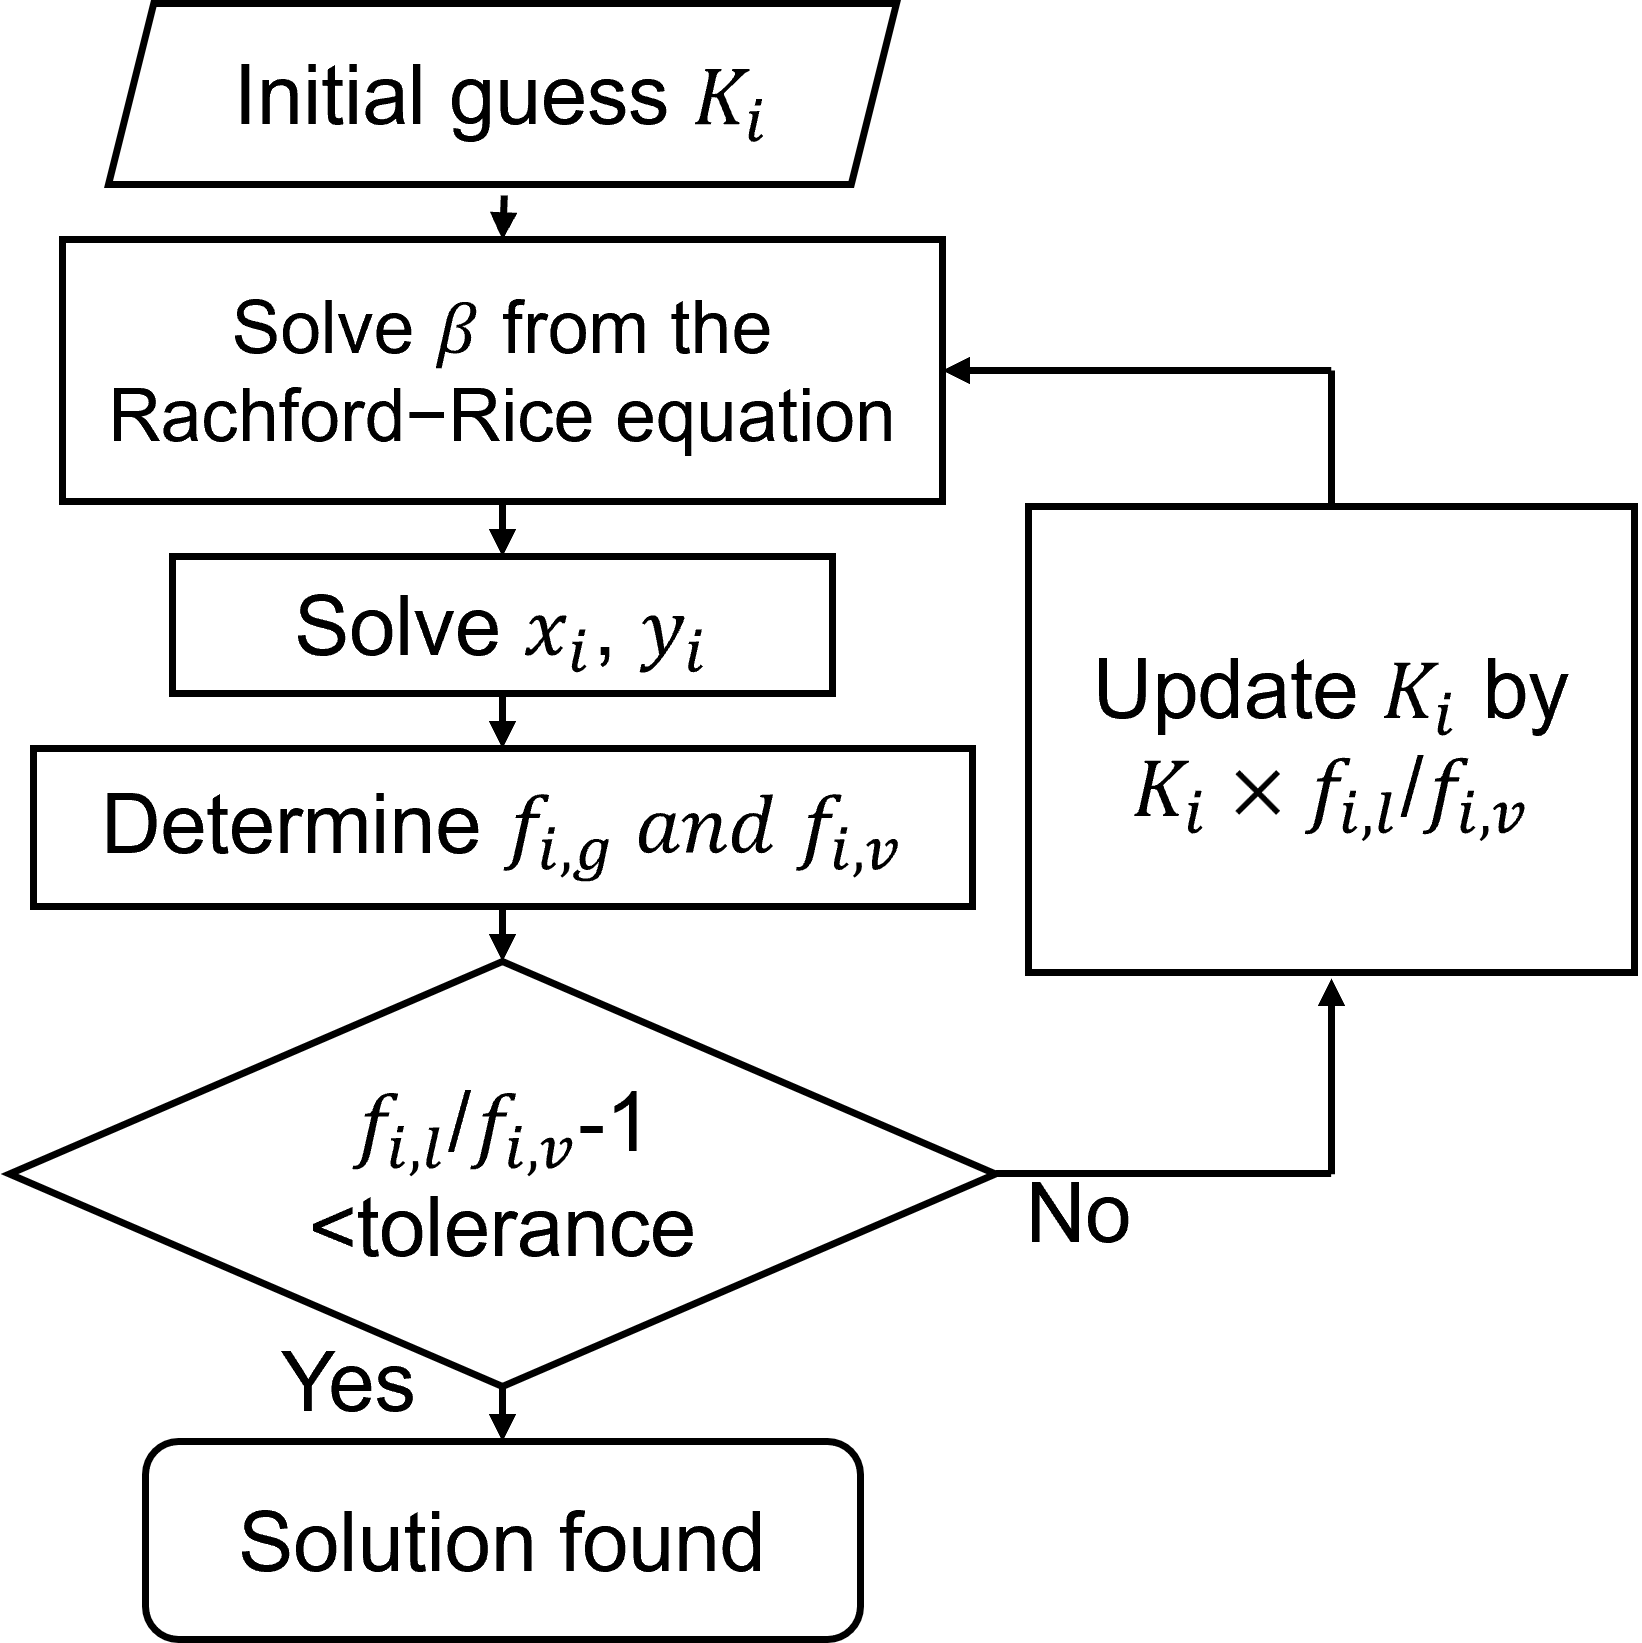
\includegraphics[width=0.35\linewidth]{TPn_flowchart.png}
\caption{Flow chart of TP flash solution process.}
\label{FC} 
\end{figure}

Once the initial guess is obtained, we proceed to solve the Rachford-Rice equation (Eq.~\ref{eq:5}) using the Newton-Raphson iteration method to determine the vapor mole fraction $\beta$. Subsequently, $x_i$ and $y_i$ can be calculated using Eqs.~\ref{eq:5-2}. The next step involves evaluating the fugacity using Eq.~\ref{fuga} and examining whether fugacity equilibrium has been achieved (i.e., $\left|f_{i,l}/f_{i,g}-1\right| < tol $). If equilibrium has not been reached, we update the equilibrium constant $K_i$ by multiplying it with the fugacity ratio $K_i=K_i \times f_{i,l}/f_{i,g}$ and then return to the step of solving the Rachford-Rice equation once again. This iterative process continues until the error falls below a specified tolerance $tol$, and $tol$ is $10^-8$ in this work. 


\textbf{PV flash and UV flash:}
The PV flash and UV flash solvers are developed based on the TP flash method, utilizing iteration methods. For both solvers, initial guesses (T for PV flash; T and P for UV flash) are obtained from the cell value in the previous time step, and a TP flash problem is solved in each iteration. During the iteration process, T and/or P are updated to find a better solution. After multiple iterations, when the error (PV flash error: $|\rho - \rho_0|$, UV flash error: $|e - e_0|$ and $|\rho - \rho_0|$) falls below a specified tolerance, the solver returns the solution of TP flash problem.


In the PV flash solver, as the pressure (P) is already provided as input, only the temperature (T) needs to be guessed and updated during the iteration. To avoid the computational cost of computing derivatives in the Newton-Raphson method, a secant method is employed to update T.


In contrast, the UV flash solver requires simultaneous guessing and updating of two variables,  temperature (T) and pressure (P), during the iteration. Therefore, the secant method cannot be directly applied. Instead, the Newton-Raphson method is used to solve UV flash problems. The required Jacobian matrix is obtained using the analytical framework described in Sec.~\ref{sec:analytical}.



\subsection{Models of transport properties}
To evaluate the dynamic viscosity and thermal conductivity at transcritical conditions, the dense fluid formulas (i.e., the Chung's method~\cite{chung1988generalized}) are used. This method gives accurate estimations of viscosity and thermal conductivity of polar, non-polar, and associating pure fluids and mixtures. 
\subsection{Viscosity}
The viscosity expressed by Chung is: 
\begin{align}
\eta = \eta_{\kappa} +\eta_p 
\end{align}
In this method, dynamic viscosity and thermal conductivity have the similar formula:
\begin{equation}
\lambda=\lambda_0 \lambda^*+\lambda_p, \label{transp}
\end{equation}
where $\lambda$ represents dynamic viscosity or thermal conductivity. $\lambda_0$ is the property at the low-pressure limit. $\lambda^*$ and $\lambda_p$ are high pressure corrections. At high pressures, $\lambda_p$ is the major contributing term compared to $\lambda_0 \lambda^*$. On the other hand, at low pressures, $\lambda^*$ is approaching unity and the $\lambda_p$ term is negligible such that Eq.~\ref{transp} reduces to $\lambda_0$. Hence, the transition between low-pressure and high-pressure properties is smoothly described by the model. 

For mass diffusivity, we used a mixture-averaged mass diffusion model~\cite{kee1996chemkin}. The mass diffusion coefficient $D_i$ of specie $i$ is defined as
\begin{equation}
D_i=\frac{1-Y_i}{\sum^N_{j\neq i}z_j/D_{j,i}},\label{massdiff}
\end{equation}
where $Y_i$ and $z_i$ are the mass and mole fractions of component $i$, respectively; $D_{i,j}$ is the binary mass diffusion coefficient of component $i$ in component $j$, which is evaluated by Fuller’s model~\cite{fuller1966new} with Takahashi’s correction~\cite{takahashi1975preparation} for high pressures.
\comment{
high-pressure (dense fluids) viscosity 
\begin{align}
& H_2 = \frac{\frac{B_1}{Y}\left(1-e^{-B_4Y}\right) +B_2G_1 e^{B_5Y}+B_3 G_1}{B_1B_4 +B_2 +B_3}
& B_{i} = b_{0,i} + b_{1,i}\omega_m + b_{2,i} \mu_{r,m}^4 + b_{3,i} \kappa_m\\
\end{align}
\begin{align}
&G_2 =\frac{ \left\{\frac{A_1}{Y} \left(1- e^{-A_4 Y}\right)+ A_2 G_1 e^{A_5 Y}+A_3 G_1 \right\}}{A_1A_4+A_2+A_3} \\ 
&Y = \frac{\rho V_{c,m}}{6M} \\
& A_{i} = a_{0,i} + a_{1,i}\omega_m + a_{2,i} \mu_{r,m}^4 + a_{3,i} \kappa_m\\
& V_{c,m}=\left(\frac{\sigma_m}{0.809}\right)^3 \\
& T^* = \frac{kT}{\epsilon_m}\\
& T_{c,m}=\frac{1.2593 \epsilon_m}{k}\\
&G_1 = \frac{1-0.5 Y }{(1-Y)^3} \\
& \omega_m = \frac{\sum_i\sum_j x_ix_j \omega_{ij}\sigma_{ij}^3}{\sigma_m^3}\\
& \mu_{r,m}= \frac{131.3 \mu_m}{\sqrt{V_{c,m}T_{c,m}}}\\
& \kappa_m = \sum_i\sum_j x_i x_j \kappa_{ij}\\
& \sigma_m^3 = \sum_i\sum_j x_i x_j \sigma_{ij}^3\\
& \frac{\epsilon_m}{k} = \frac{\sum_i\sum_j x_i x_j\left(\frac{\epsilon_{ij}}{k}\right) \sigma_{ij}^3}{\sigma_m^3 }\\
& \omega_{ij} = \frac{\omega_i+\omega_j}{2}\\
& \sigma_{ij} = \xi_{ij} \sqrt{\sigma_i \sigma_j}\\
& \mu_m^4 = \left(\sum_i\sum_j x_i x_j \mu_{i}^2 \mu_{j}^2  \frac{k}{\epsilon_{ij}\sigma_{ij}^3}\right) \sigma_m^3\frac{\epsilon_m}{k}\\
& \kappa_{ij} = \sqrt{\kappa_i \kappa_j}\\
& \frac{\epsilon_{ij}}{k} = \zeta_{ij} \sqrt{ \frac{\epsilon_{i}}{k} \frac{\epsilon_{j}}{k}}\\
& \sigma_i = 0.809 V_{c,i}^{1/3}\\
& \frac{\epsilon_i}{k} = \frac{T_{c,i}}{1.2593}\\
&\lambda = \lambda_{\kappa} +\lambda_p \\
&\lambda_{\kappa} = \lambda_0 \left( \frac{1}{H_2}+B_6 Y \right) \\
&\lambda_p = 3.039\times 10^{-4}\frac{\sqrt{\frac{ T_{c,m}}{M}}}{V_{c,m}^{2/3}}B_7Y^2H_2 \sqrt{\frac{T}{T_{c,m}}}\\
& \lambda_0=7.452 \frac{\eta_0\Psi}{M}\\
& \Psi = 1 +\alpha\frac{0.215 + 0.2828\alpha-1.061\beta+0.2665Z }{0.6366 +\beta Z +1.061\alpha \beta }\\
& \alpha = \frac{C_v}{R} -\frac{3}{2}\\
& \beta = 0.7862 - 0.7109 \omega_m + 1.3168 \omega_m^2\\
& Z =2.0+10.5 \left(\frac{T}{T_{c,m}}\right)^2\\
\end{align}
$\kappa$ is a correction factor for hydrogen-bonding effect, for water $\kappa=0.075 908$
$\mu$ is dipole moment,
$\xi_{ij}$ and $\zeta_{ij}$ are unity
$\omega$  acentric factor
$A = 1.16145, B = 0.14874, C = 0.52487, D = 0.77320, E = 2.16178, F = 2.43787, G = -6.435\times 10^{-4}, H = 7.273 71, S = 18.0323$, and $W = -0.768 30$.

\begin{table}
    \caption{The initial condition of temporal mixing layer.}\label{TML_init_table2}
    \begin{threeparttable} 
\begin{tabular*}{0.8\textwidth}{@{} l|lllll@{}}
    \toprule
    i     & $a_{0,i}$   & $a_{1,i}$  & $a_{2,i}$   & $a_{3,i}$ \\
    \midrule
    1     & 6.32402          & 50.41190          & -51.68010       & 1189.02000  \\
    2     & 0.0012102        & -0.0011536        & -0.0062571      & 0.037283    \\
    3     & 5.28346          & 254.20900         & -168.48100      & 3898.27000  \\
    4     & 6.62263          & 38.09570          & -8.46414        & 31.41780    \\
    5     & 19.74540         & 7.63034           & -14.35440       & 31.52670    \\
    6     & -1.89992         & -12.53670         & 4.98529         & -18.15070   \\
    7     & 24.27450         & 3.44945           & -11.29130       & 69.34660    \\
    8     & 0.79716          & 1.11764           & 0.012348        & -4.11661    \\
    9     & -0.23816         & 0.067695          & -0.81630        & 4.02528     \\
    10    & 0.068629         & 0.34793           & 0.59256         & -0.72663    \\
    \bottomrule
\end{tabular*}
\begin{tablenotes}
    \footnotesize    
    \item Subscripts T and B refer to Top and Bottom, respectively. $L_y = 0.6\times L_x$,  $Re_0=1000$. Mesh in the center subdomain is $256\times 152 \times 256$, and the top and bottom subdomain mesh is $256\times 152\times 64$. $P = 50$ bar, $T_B=293$ K, $M_c = 0.3$, $A_i = 0.25, 0.5, 1$, $B_i = 0.05, 0, 1$, and $F_{2D}= F_{3D} = 0.05$.\\
  \end{tablenotes}
\end{threeparttable}
\end{table}


\begin{table}
    \caption{The initial condition of temporal mixing layer.}\label{TML_init_table1}
    \begin{threeparttable} 
\begin{tabular*}{0.8\textwidth}{@{} l|lllll@{}}
    \toprule
    i     & $b_{0,i}$   & $b_{1,i}$  & $b_{2,i}$   & $b_{3,i}$ \\
    \midrule
    1     & 2.41657          & 0.74824           & -0.91858        & 121.72100  \\
    2     & -0.50924         & -1.50936          & -49.99120       & 69.98340   \\
    3     & 6.61069          & 5.62073           & 64.75990        & 27.03890  \\
    4     & 14.54250         & -8.91387          & -5.63794        & 74.34350    \\
    5     & 0.79274          & 0.82019           & -0.69369        & 6.31734    \\
    6     & -5.86340         & 12.80050          & 9.58926         & -65.52920   \\
    7     & 81.17100         & 114.15800         & -60.84100       & 466.77500   \\
 \bottomrule
\end{tabular*}
\begin{tablenotes}
    \footnotesize    
    \item Subscripts T and B refer to Top and Bottom, respectively. $L_y = 0.6\times L_x$,  $Re_0=1000$. Mesh in the center subdomain is $256\times 152 \times 256$, and the top and bottom subdomain mesh is $256\times 152\times 64$. $P = 50$ bar, $T_B=293$ K, $M_c = 0.3$, $A_i = 0.25, 0.5, 1$, $B_i = 0.05, 0, 1$, and $F_{2D}= F_{3D} = 0.05$.\\
  \end{tablenotes}
\end{threeparttable}
\end{table}

\begin{align}
T^* = 1.2593 \frac{T}{T_c}
\end{align}


}

%%%%%%%%%%%%%%%%%%%%%%%%%%%%%%%%%%%%%%%%%%%%%%%%%%%%%%%%%%%%%%%%%%%%%%%%%%%%%%%%
